\documentclass{article}
  \usepackage[total={8cm,21cm},top=2cm, left=2cm]{geometry}
  %Paquetes adicionales
  \usepackage{latexsym,amsmath,amssymb,amsfonts}
  \usepackage[latin1]{inputenc}
  \usepackage[T1]{fontenc}
  \usepackage{graphicx}
  \usepackage{caption}
  \usepackage[spanish]{babel} % Idioma espa�ol

\usepackage{wrapfig} %Figuras al lado de texto
\usepackage[rflt]{floatflt} %Figuras flotantes entre el texto

\begin{document} 

\begin{floatingfigure}[r]{4.5cm}
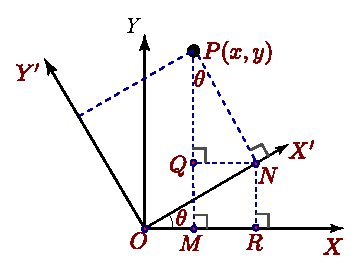
\includegraphics{images/figura4}
\captionof{figure}{Una figura}
\end{floatingfigure}

\end{document}